\chapter{贝叶斯网络}

贝叶斯网络(Bayesian network),又称信念网络(Belief Network),或有向无环图模型(directed acyclic graphical model),是一种概率图模型,于1985年由Judea Pearl首先提出。它是一种模拟人类推理过程中因果关系的不确定性处理模型,其网络拓朴结构是一个有向无环图(DAG)。我们将有因果关系(或非条件独立)的变量或命题用箭头来连接(换言之,连接两个节点的箭头代表此两个随机变量是具有因果关系,或非条件独立)。若两个节点间以一个单箭头连接在一起,表示其中一个节点是“因(parents)”,另一个是“果(children)”,两节点就会产生一个条件概率值。 例如,假设节点E直接影响到节点H,即E→H,则用从E指向H的箭头建立结点E到结点H的有向弧(E,H),权值(即连接强度)用条件概率P(H|E)来表示,如下图所示:

\begin{figure}[H]
    \centering
    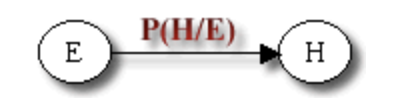
\includegraphics[scale=0.5]{figures/贝叶斯网络概述.png}
    \caption{贝叶斯网络}
\end{figure}

\subsection*{主要历程}

\begin{figure}[H]
    \centering
    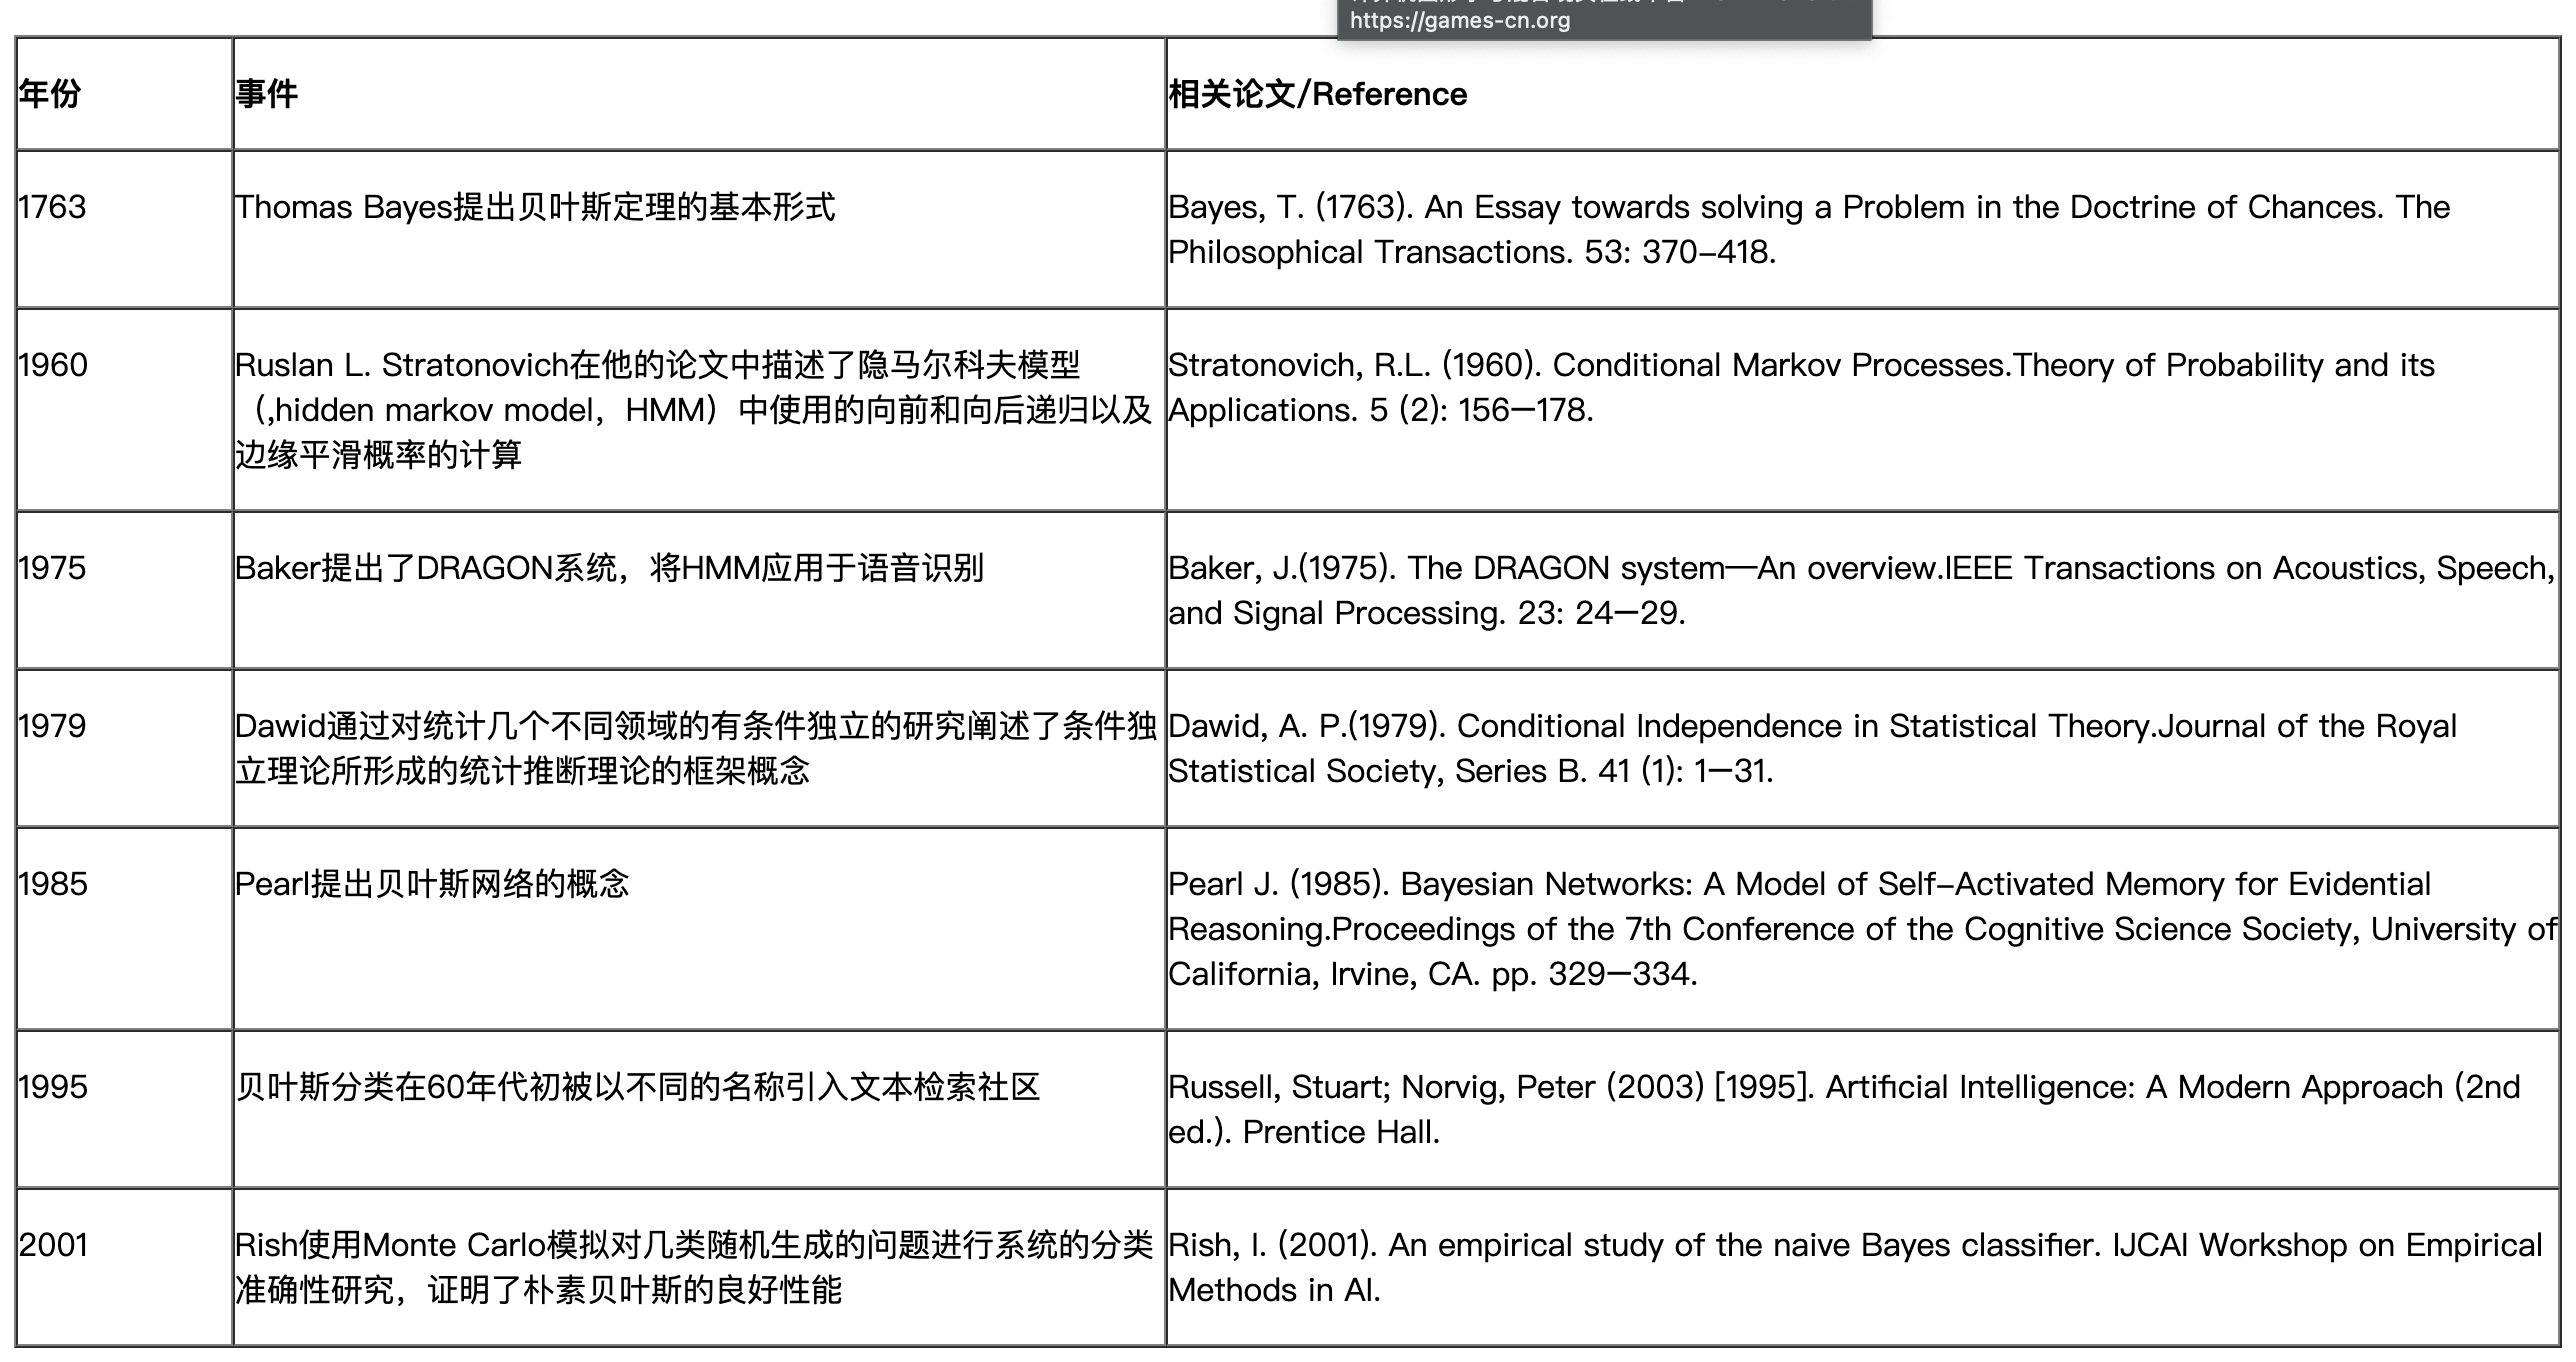
\includegraphics[scale=0.16]{figures/贝叶斯网络发展主要事件.png}
    \caption{贝叶斯网络发展主要事件}
\end{figure}

\section{贝叶斯公式与乘法定理}

\subsection*{乘法定理}

事件$A$在事件$B$发生的情况下发生的条件概率表示为
\begin{equation}
    P(A|B)=\frac{P(AB)}{P(B)}
\end{equation}

因此乘法定理写成
\begin{equation}
    P(AB)=P(A|B)P(B)
\end{equation}

\subsection*{贝叶斯公式}

贝叶斯公式可以理解成:\textsl{后验概率 = (似然性*先验概率)/标准化常量},数学表达为
\begin{equation}
    P(A|B)=\frac{P(AB)}{P(B)}=\frac{P(A)P(B|A)}{P(B)}
\end{equation}

\subsection*{链式法则}

对于非相互独立的随机事件的乘法是相对复杂的,根据乘法定理,我们可以得到n个随机变量的联合概率
\begin{equation}
    P(x_1,\cdots,x_n)=P(x_1)P(x_2|x_1)\cdots P(x_n|x_{n-1},\cdots,x_1)
\end{equation}

举个例子:假设事件$X_1,X_2,X_3$三个事件,联合概率分布为
\begin{equation}
    P(X_1X_2X_3)=P(X_1)P(X_2|X_1)P(X_3|X_1X_2)
\end{equation}

可以发现$P(X_1)P(X_2|X_1)=P(X_1X_2)$,这刚好就是$X_1X_2$同时发生的概率,也就是$P(X_3|X_2X_1)$中
的条件。

\section{贝叶斯网络}

贝叶斯网络用有向图来描述$n$个随机事件的概率分布,假设事件$a$发生情况下$b$发生的概率为$p(b|a)$,$b$发生情况下$c$发生的概率为$p(c|b)$,
$a$发生的情况下$c$发生的条件概率表示为$p(c|a)$,通过有向图表述为
\begin{figure}[H]
    \centering
    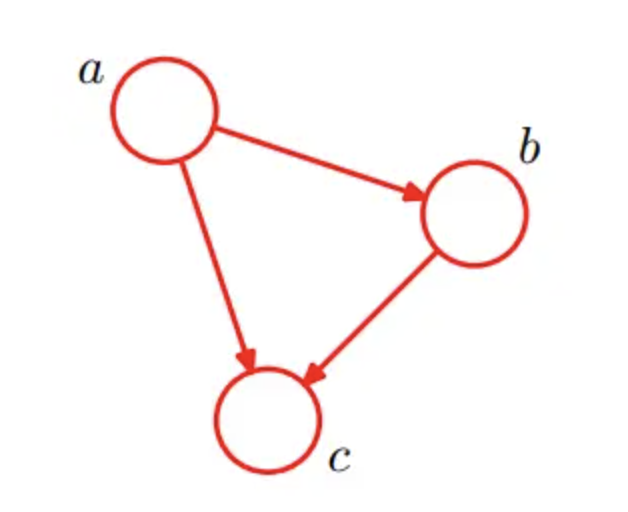
\includegraphics[scale=0.2]{figures/abc贝叶斯网络.png}
    \caption{事件abc的贝叶斯网络}
\end{figure}

图的节点表示事件,图的边表示条件概率。从图中可以看到因为$a$导致$b$,$a$和$b$导致$c$,所以有
\begin{equation}
    P(abc)=P(a)P(b|a)P(c|ba)
\end{equation}

下图是一个贝叶斯网络的一般形态。

\begin{figure}[H]
    \centering
    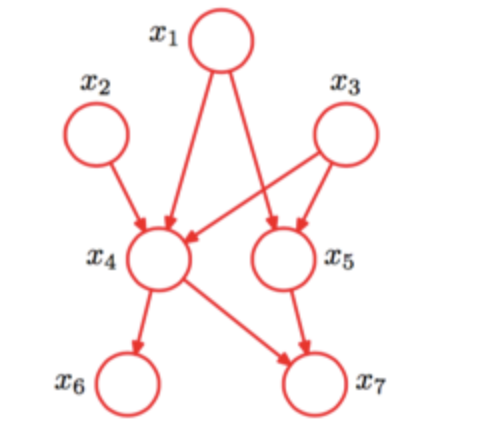
\includegraphics[scale=0.6]{figures/全链接贝叶斯网络.png}
    \caption{一个"正常"的贝叶斯网络}
\end{figure}

\section{条件独立性}

如果事件$A$和事件$B$是相互独立的,则乘法公式满足
\begin{equation}
    P(AB)=P(A)P(B)
\end{equation}

贝叶斯网络结构暗示条件独立性。例如如下简单的贝叶斯网络

\begin{figure}[H]
    \centering
    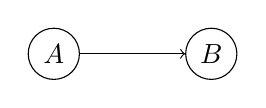
\begin{tikzpicture}
        \node[circle,draw = black,fill = white,inner sep = 0pt,minimum size = 0.65cm] (A) at (0, 0) {{$A$}};
        \node[circle,draw = black,fill = white,inner sep = 0pt,minimum size = 0.65cm] (B) at (2, 0) {{$B$}};
        \path [draw, ->] (A) edge (B);
    \end{tikzpicture}
    \caption{$A$导致$B$,$A$和$B$存在因果关系,因此不存在条件独立性}
\end{figure}

联合概率分布为
\begin{equation}
    P(AB)=P(A)P(B|A)
\end{equation}

如果$A$和$B$是相互独立的两个事件
\begin{figure}[H]
    \centering
    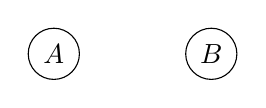
\begin{tikzpicture}
        \node[circle,draw = black,fill = white,inner sep = 0pt,minimum size = 0.65cm] (A) at (0, 0) {{$A$}};
        \node[circle,draw = black,fill = white,inner sep = 0pt,minimum size = 0.65cm] (B) at (2, 0) {{$B$}};
    \end{tikzpicture}
    \caption{$A$和$B$不存在因果关系,即体现条件独立性}
\end{figure}

此时概率分布就是相对独立事件的乘法公式。

\subsection*{条件独立性的判定}

对于一般性的贝叶斯网络我们如何去判定节点之间的条件独立性呢?考虑一下三种贝叶斯网络的结构在什么情况下能推出$P(AB)=P(A)P(B)$
\begin{framed}
\begin{enumerate}[itemindent=2em]
    \item \textcolor{MSBlue}{\textsl{tail-to-tail:父节点已知则子节点独立}}:;
    
    \begin{figure}[H]
        \centering
        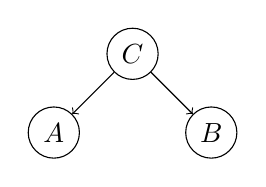
\begin{tikzpicture}
            \node[circle,draw = black,fill = white,inner sep = 0pt,minimum size = 0.65cm] (A) at (0, 0) {{$A$}};
            \node[circle,draw = black,fill = white,inner sep = 0pt,minimum size = 0.65cm] (B) at (2, 0) {{$B$}};
            \node[circle,draw = black,fill = white,inner sep = 0pt,minimum size = 0.65cm] (C) at (1, 1) {{$C$}};
            \path[draw,->] (C) edge (A);
            \path[draw,->] (C) edge (B);
        \end{tikzpicture}
        \caption{$C$未知,$A$和$B$被$C$的影响,所以不独立}
    \end{figure}

    如果$C$发生的概率未知,根据贝叶斯网络结构,联合概率分布为
    \begin{equation}
        P(ABC)=P(C)P(A|C)P(B|C)
    \end{equation}

    由于不知道$P(C)$,无法得出$P(AB)=P(A)P(B)$。

    如果$C$发生的概率已知,那么根据$P(AB|C)=P(ABC)/P(C)$\footnote{原来$P(C)$和$P(ABC)$都是未知,所以$P(AB|C)$也未知,$P(C)$已知的情况下相当于可以把$P(ABC)$表示成$P(AB|C)$},联合概率分布为
    \begin{equation}
        P(AB|C)=P(A|C)P(B|C)
    \end{equation}

    所以此时$A$和$B$的条件独立。所以,在$C$给定的条件下,$A$、$B$被阻断(blocked),是独立的,称之为\textsl{tail-to-tail条件独立}。
    \begin{figure}[H]
    \centering
    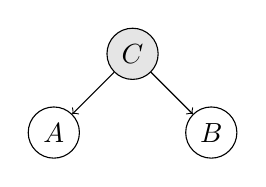
\begin{tikzpicture}
        \node[circle,draw = black,fill = white,inner sep = 0pt,minimum size = 0.65cm] (A) at (0, 0) {{$A$}};
        \node[circle,draw = black,fill = white,inner sep = 0pt,minimum size = 0.65cm] (B) at (2, 0) {{$B$}};
        \node[circle,draw = black,fill = gray!20,inner sep = 0pt,minimum size = 0.65cm] (C) at (1, 1) {{$C$}};
        \path[draw,->] (C) edge (A);
        \path[draw,->] (C) edge (B);
    \end{tikzpicture}
    \caption{若$C$是先验概率,$A$和$B$之间被$C$阻断,因此不存在因果关系,即$A$和$B$条件独立}
    \end{figure}

    \item \textcolor{MSBlue}{\textsl{head-to-tail:中间节点已知则两边节点独立}};

    \begin{figure}[H]
        \centering
        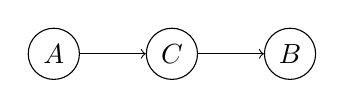
\begin{tikzpicture}
            \node[circle,draw = black,fill = white,inner sep = 0pt,minimum size = 0.65cm] (A) at (0, 0) {{$A$}};
            \node[circle,draw = black,fill = white,inner sep = 0pt,minimum size = 0.65cm] (C) at (1.5, 0) {{$C$}};
            \node[circle,draw = black,fill = white,inner sep = 0pt,minimum size = 0.65cm] (B) at (3, 0) {{$B$}};
            \path[draw,->] (A) edge (C);
            \path[draw,->] (C) edge (B);
        \end{tikzpicture}
        \caption{$C$的概率未知的情况下,$A$可以通过$C$去影响$B$,因此$A$和$B$存在因果关系}
    \end{figure}

    联合概率分布为
    \begin{equation}
        P(ABC)=P(A)P(C|A)P(B|C)
    \end{equation}

    $C$的概率未知的情况下,$A$可以通过$C$去影响$B$,因此$A$和$B$存在因果关系。

    如果已知$C$发生的概率$P(C)$,根据\textsl{贝叶斯公式}
    \begin{equation}
        \begin{aligned}
            & P(ABC)=P(A)P(C|A)P(B|C)\\
            & \Rightarrow P(AB|C)=\frac{P(ABC)}{P(C)}=\frac{P(A)P(C|A)P(B|C)}{P(C)}\\
            &  \Rightarrow P(AB|C)=\frac{P(ABC)}{P(C)}=\frac{P(AC)P(B|C)}{P(C)}\\
            & \Rightarrow P(AB|C)=P(A|C)P(B|C)
        \end{aligned}
    \end{equation}

    这相当于$C$已知的情况下,$A$和$B$的关系被截断了,因此$A$和$B$在$C$概率已知的情况下是条件独立的。
    \begin{figure}[H]
        \centering
        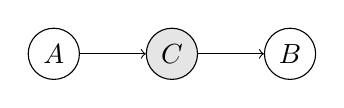
\begin{tikzpicture}
            \node[circle,draw = black,fill = white,inner sep = 0pt,minimum size = 0.65cm] (A) at (0, 0) {{$A$}};
            \node[circle,draw = black,fill = gray!20,inner sep = 0pt,minimum size = 0.65cm] (C) at (1.5, 0) {{$C$}};
            \node[circle,draw = black,fill = white,inner sep = 0pt,minimum size = 0.65cm] (B) at (3, 0) {{$B$}};
            \path[draw,->] (A) edge (C);
            \path[draw,->] (C) edge (B);
        \end{tikzpicture}
        \caption{$C$是先验概率,$A$和$B$之间被$B$阻断,因此不存在因果关系,即$A$和$B$条件独立}
    \end{figure}

    \item \textcolor{MSBlue}{\textsl{head-to-head:子节点未知则父节点独立} };
    
    \begin{figure}[H]
        \centering
        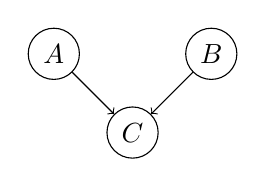
\begin{tikzpicture}
            \node[circle,draw = black,fill = white,inner sep = 0pt,minimum size = 0.65cm] (A) at (0, 0) {{$A$}};
            \node[circle,draw = black,fill = white,inner sep = 0pt,minimum size = 0.65cm] (C) at (1, -1) {{$C$}};
            \node[circle,draw = black,fill = white,inner sep = 0pt,minimum size = 0.65cm] (B) at (2, 0) {{$B$}};
            \path[draw,->] (A) edge (C);
            \path[draw,->] (B) edge (C);
        \end{tikzpicture}
        \caption{$C$是先验概率,$A$和$B$之间被$B$阻断,因此不存在因果关系,即$A$和$B$条件独立}
    \end{figure}

    $C$概率未知的情况下,贝叶斯网络的联合概率分布为
    \begin{equation}
        P(ABC)=P(A)P(B)P(C|AB)
    \end{equation}

    因为$P(C|AB)$和$P(A)$和$P(B)$独立性无关,所以可以简化为
    \begin{equation}
        P(AB)=P(A)P(B)
    \end{equation}

    如果$P(C)$给定,则
    \begin{equation}
        P(AB|C)=\frac{P(A)P(B)P(C|AB)}{P(C)}
    \end{equation}

    上面式子因为约不掉$P(C)$,所以没办法推出$P(AB)=P(A)P(B)$,因此不满足条件独立性。

    因此在head to head的情况下,如果没有观测到共同子节点$C$的概率,则父节点$A$和$B$相互独立,反之则不满足独立条件。

    \begin{figure}[H]
        \centering
        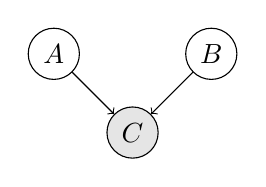
\begin{tikzpicture}
            \node[circle,draw = black,fill = white,inner sep = 0pt,minimum size = 0.65cm] (A) at (0, 0) {{$A$}};
            \node[circle,draw = black,fill = gray!20,inner sep = 0pt,minimum size = 0.65cm] (C) at (1, -1) {{$C$}};
            \node[circle,draw = black,fill = white,inner sep = 0pt,minimum size = 0.65cm] (B) at (2, 0) {{$B$}};
            \path[draw,->] (A) edge (C);
            \path[draw,->] (B) edge (C);
        \end{tikzpicture}
        \caption{$C$是先验概率,$C$已知的情况下父节点通过子节点关联,$A$和$B$条件不独立}
    \end{figure}

\end{enumerate}

\end{framed}


可以这么理解:老父亲还在,则兄弟关系还在,老父亲出问题了,兄弟联系断了。如果两个节点是直接连接的,它们肯定是非条件独立的,
是直接因果关系。其中父节点是“因”,子节点是“果”。


\subsection*{条件独立性的意义}

条件独立性可以简化链过长;条件独立性允许将复杂的联合概率分布分解成更简单的条件概率分布。在实际应用中,计算高维联合概率分布是非常困难的,
而条件独立性提供了简化这些计算的方法。例如,在贝叶斯网络(Bayesian Network)中,通过利用条件独立性,联合概率分布$P(X_1,X_2,\cdots,X_N)$
可以分解为一系列的条件概率:

\begin{eqnarray}
    P(X_1,X_2,\cdots,X_N)=\prod\limits_{i=1}^{N} P(X_i|\pi(X_i))
\end{eqnarray}

其中$\pi(X_i)$表示$X_i$的父节点集合。利用条件独立性关系,这种分解显著降低了计算复杂度。
\begin{figure}[H]
    \centering
    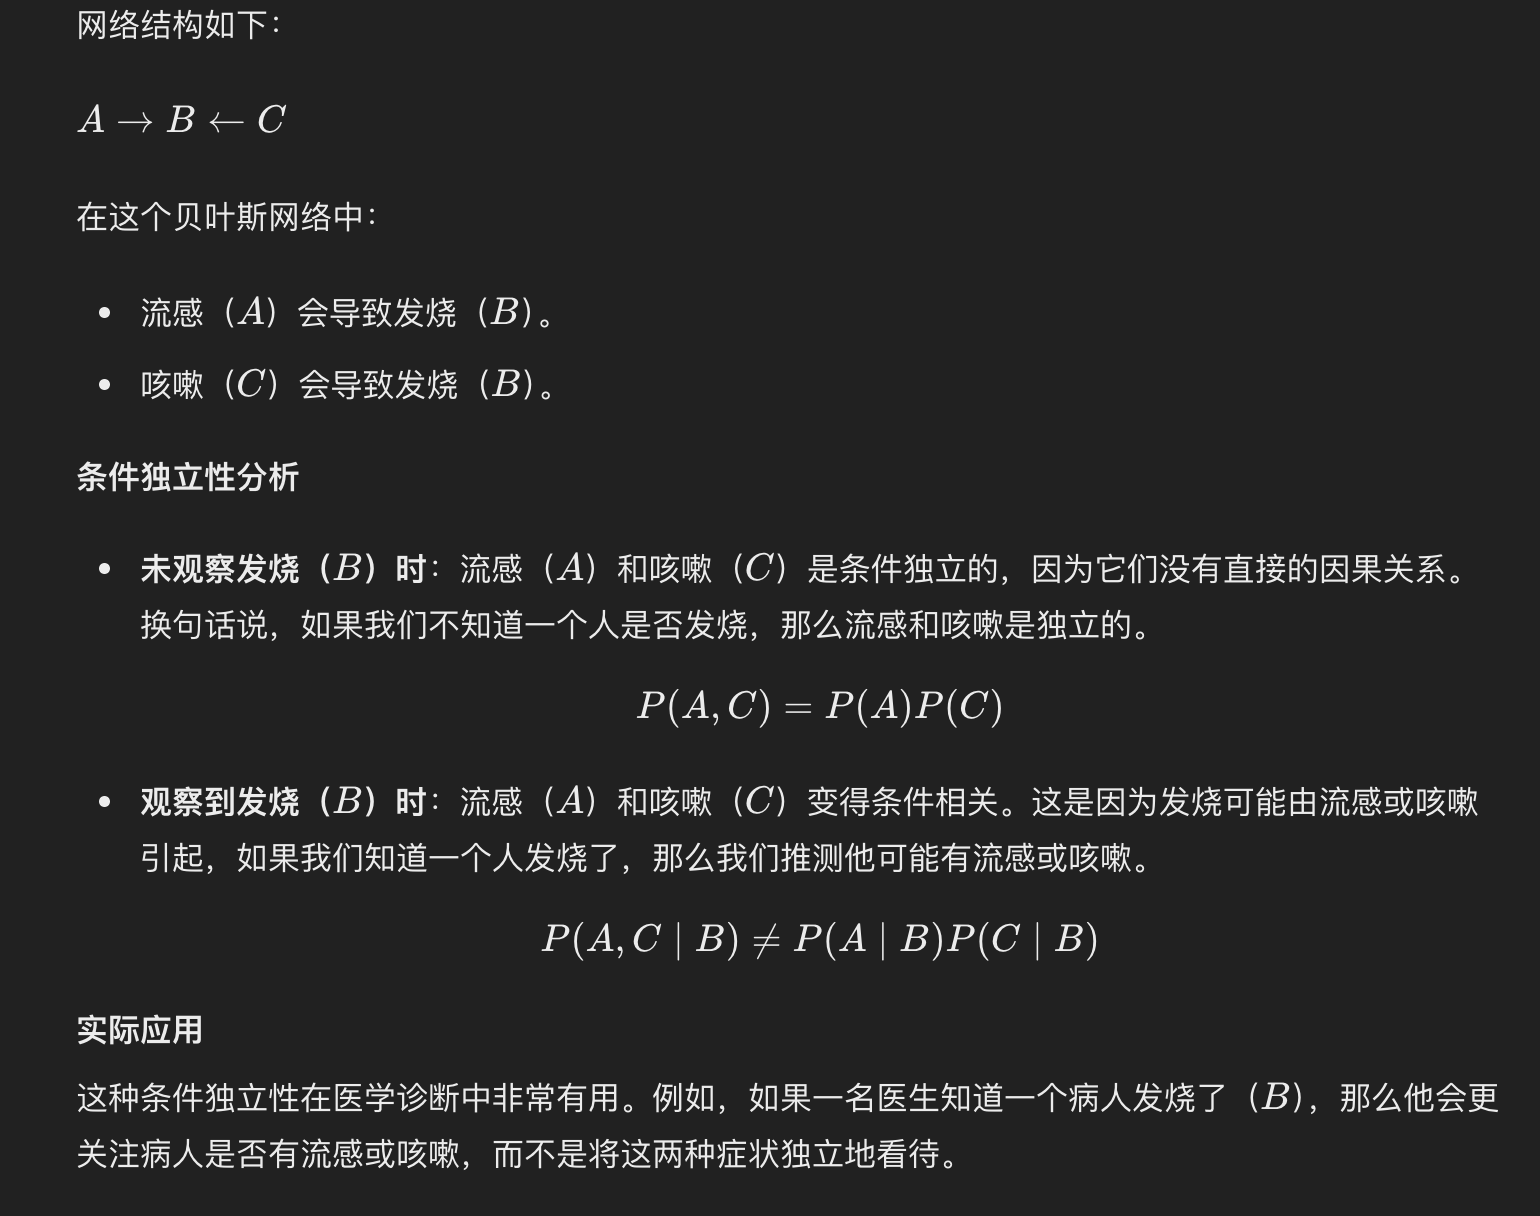
\includegraphics[scale=0.25]{figures/贝叶斯网络gpt给的例子.png}
    \caption{chat-GPT给的例子}
\end{figure}

\section{D-Separation算法}

$D$分离算法又称为有向分离算法,是一种用来判断变量是否条件独立的图形化方法。对于一个DAG,D分离可以快速判断两个节点之间是否条件独立。

在前面小节中已经列举了\textsl{条件独立性判定}可能的三种情况:\textsl{tail-to-tail}、\textsl{head-to-tail}、\textsl{head-to-head},
基于三种条件独立性判定情况,$D$分离算法通过路径遍历来确定是否路径被阻断。下面举例子说明

\subsection*{例子}

\subsection*{马尔可夫毯}

对于一个人来讲和全世界的关系等于和自己周围的血缘关系,和别人没关系;

\section{贝叶斯网络在机器学习中的应用}

\section{贝叶斯网络模型}

\subsection*{朴素贝叶斯(Native Bayes)}
单一;

贝叶斯假设
\begin{equation}
    P(X|Y)=\prod\limits_{i=1}^{K}p(x_i|y=1)
\end{equation}

概率图模型

\subsection*{高斯混合模型}

\subsection*{和时间相关的}

主要两个算法:\textsl{Markcov Chain}和\textsl{高斯过程(无限维高斯分布)}

\subsection*{连续的}

\textsl{高斯贝叶斯网络}

\subsection*{动态系统}

混合和时间,最常见的是HMM,LDS,

